\LaTeX{} is een softwaresysteem dat je kan vergelijken met een tekstverwerker zoals Microsoft Word. Het is zeer populair in de wetenschappelijke wereld, want het blinkt uit in het maken van technische documenten. Het idee van \LaTeX{} is WYMIWYG, "What you mean is what you get", en dus een markup\hyp{}taal.

Als eerst kwam ik in contact met \LaTeX{} door de tekstverwerker van MacOS, genaamd Pages. Hier kun je wiskundige formules invoegen via \LaTeX{}. Eerst kopieerde ik formules die ik online vond of ik converteerde ze via een online converter. Daarna zag ik dat de taal niet zo moeilijk te begrijpen was en zo kon ik mijn eigen formules uitschrijven.

Later kwam ik er achter dat \LaTeX{} niet enkel gemaakt is voor wiskundige formules weer te geven, maar ook kan gebruikt worden als een volwaardige tekstverwerker. Omdat het zeer veel gebruikt wordt om papers mee te schrijven, had ik besloten om mijn eindwerk hiermee te schrijven.

\LaTeX{} is het meest gebruikte pakket met macro's voor \TeX{}. \TeX{} is eind jaren 70 ontwikkeld door Donald Knuth, om op een relatief eenvoudige manier het beschrijven van een ingewikkelde lay\hyp{}out mogelijk te maken. \TeX{} werkt zoals een computerprogramma, eerst moet de broncode geschreven worden om nadien gecompileerd te worden en een zo een resultaat te krijgen. Meestal wordt er gecompileerd naar een pdf\hyp{}bestand.

De macro's die in het \LaTeX\hyp{}pakket zitten, zijn gemaakt om veel gebruikte zaken te defini\"eren om het opmaakprocess te versnellen. Zo moet de schrijver minder macro's zelf gaan schrijven, maar de mogelijkheid tot eigen macro's en het aanpassen van de bestaande is nog aanwezig.

Het hele idee achter het opmaken in \LaTeX{} is dat je op voorhand bepaalde regels definieerd en je gedurende het schrijfproces je hier geen rekening meer mee moet houden. Zo krijg je een heel consistente lay\hyp{}out doorheen je bestand. Het wijzigen van de lay\hyp{}out, moet in principe ook maar op één globale locatie gebeuren en alles volgt deze regels.

Als oefening begon ik met de templates van de benodigde documenten om te vormen naar een \LaTeX\hyp{}formaat, zoals het stageportfolio, de projectomschrijving en uiteindelijk ook het eindwerk zelf. Door meer en meer met deze taal te werken, kwam ik op conventies en veranderde ik de gehele structuur van de voordien gemaakte documenten.

\LaTeX{} heeft in mijn mening een redelijk stijle leercurve, maar als hier hier eenmaal over bent kan je er de vruchten van plukken. Zo heb ik wat meer tijd gedaan over de opmaak van mijn stageportfolio en de projectomschrijving, maar voor mijn eindwerk en iTalent portfolio heb ik zeer veel tijd gewonnen en mij praktisch niet meer moeten bezig houden met de opmaak.

\begin{figure}[!h]
    \centering
    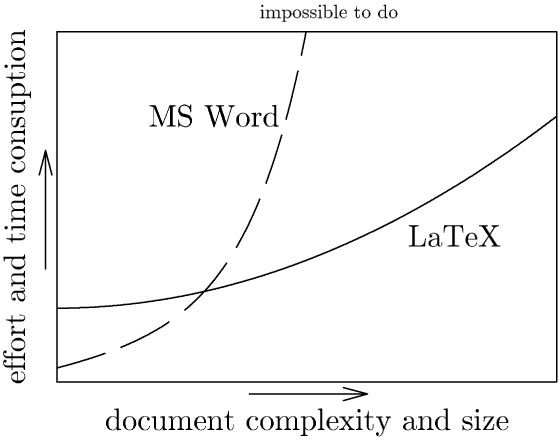
\includegraphics[width=0.44\linewidth]{latex/ms_word_vs_latex.png}
  \end{figure}

Het hele idee achter mijn eindwerk schrijven in \LaTeX{} was dat ik na mijn bachelor nog wou doorschakelen naar een master. Hier zou ik dat een master thesis moeten schrijven, om mij zo veel mogelijk te kunnen concentreren op het effectief schrijven en niet zo zeer op de opmaak dacht ik deze in \LaTeX{} te schrijven. En omdat heel veel master thesissen in \LaTeX{} geschreven worden leek mij dit ook de correcte oplossing.

Nog een groot voordeel is kunnen gebruiken van Bib\TeX{}, dit is een soort van extentie om het aan te leggen van literatuurlijsten binnen \LaTeX. Google Scholar, gebruikt om bronnen op te zoeken, heeft een handige functie waarmee je gezochte bronnen kan citeren in Bib\TeX\hyp{}formaat. Zo moet er zelf niet naar bepaalde informatie gezocht worden op een website die je wilt citeren.

Het leren van \LaTeX{} is voor mij zeer nuttig geweest. Ik heb een andere kijk gekregen voor het maken en opstellen van tekstdocumenten. Ik verlies in het algemeen veel minder tijd met het opmaken en verfijnen van de opmaak. Hierdoor heb ik meer tijd om mij bezig te houden met de tekst uit te schrijven. De documenten die ik schrijf zijn overzichtelijker om te maken en lezen.

Doordat ik nieuwsgierig ben van aard, ga ik snel nieuwe technologi\"en onderzoeken en leren. Dit zodat ik mijn eigen blijf ontwikkelen en blijf groeien als informaticus. Mijn doel is zo performant mogelijk werken, dus zo weinig mogelijk tijd verliezen met zaken die eigenlijk niet nodig zijn.

Ik vind het ook spannend om nieuwe zaken te leren. Vaak haal ik er dingen uit die ik op voorhand niet had verwacht, bijvoorbeeld op oplossen van bepaalde problemen of het automatiseren van taken. Daarom dat in mijn ogen eigen projecten maken het meest effectieve is om nieuwe zaken bij te leren. Want je kiest zelf voor dat project en je bent er dus ook gemotiveerd om hiervoor te werken. En je komt op problemen die je zelf moet oplossen en er geen verbetersleutel is waar je naar kan spieken.

Broncode iTalent portfolio: \url{https://github.com/VicSegers/iTalent-portfolio}